\newpage

\section*{ $^{58}$Ni(n,p)$^{58}$Co }

Power Level: 100 kW(th) \\
Time at Power: 60.0 m \\
Wait Time:  2.0 d \\
Counting Time: 60.0 m \\
Total Activity at Removal: 3.79e-02 $\mu Ci$

\begin{table*}[h]
\centering
\begin{tabular}{ |c|c|c|c|c|c| }
 \hline
 Position & Mass $mg$ & Counting Activity $\mu Ci$ & Area (Counts) & Error \% \\
 \hline 
 1 & 1.34 & 8.02e-03 & 3.01e+04 & 0.5768 \\ 
\hline
 2 & 1.34 & 1.26e-02 & 4.72e+04 & 0.4601 \\ 
\hline
 3 & 1.34 & 1.17e-02 & 4.37e+04 & 0.4783 \\ 
\hline
 4 & 1.34 & 4.94e-03 & 1.85e+04 & 0.7349 \\ 
\hline
\end{tabular}
\end{table*}

\begin{figure}[h]
\centering
\begin{subfigure}{.5\textwidth}
  \centering
     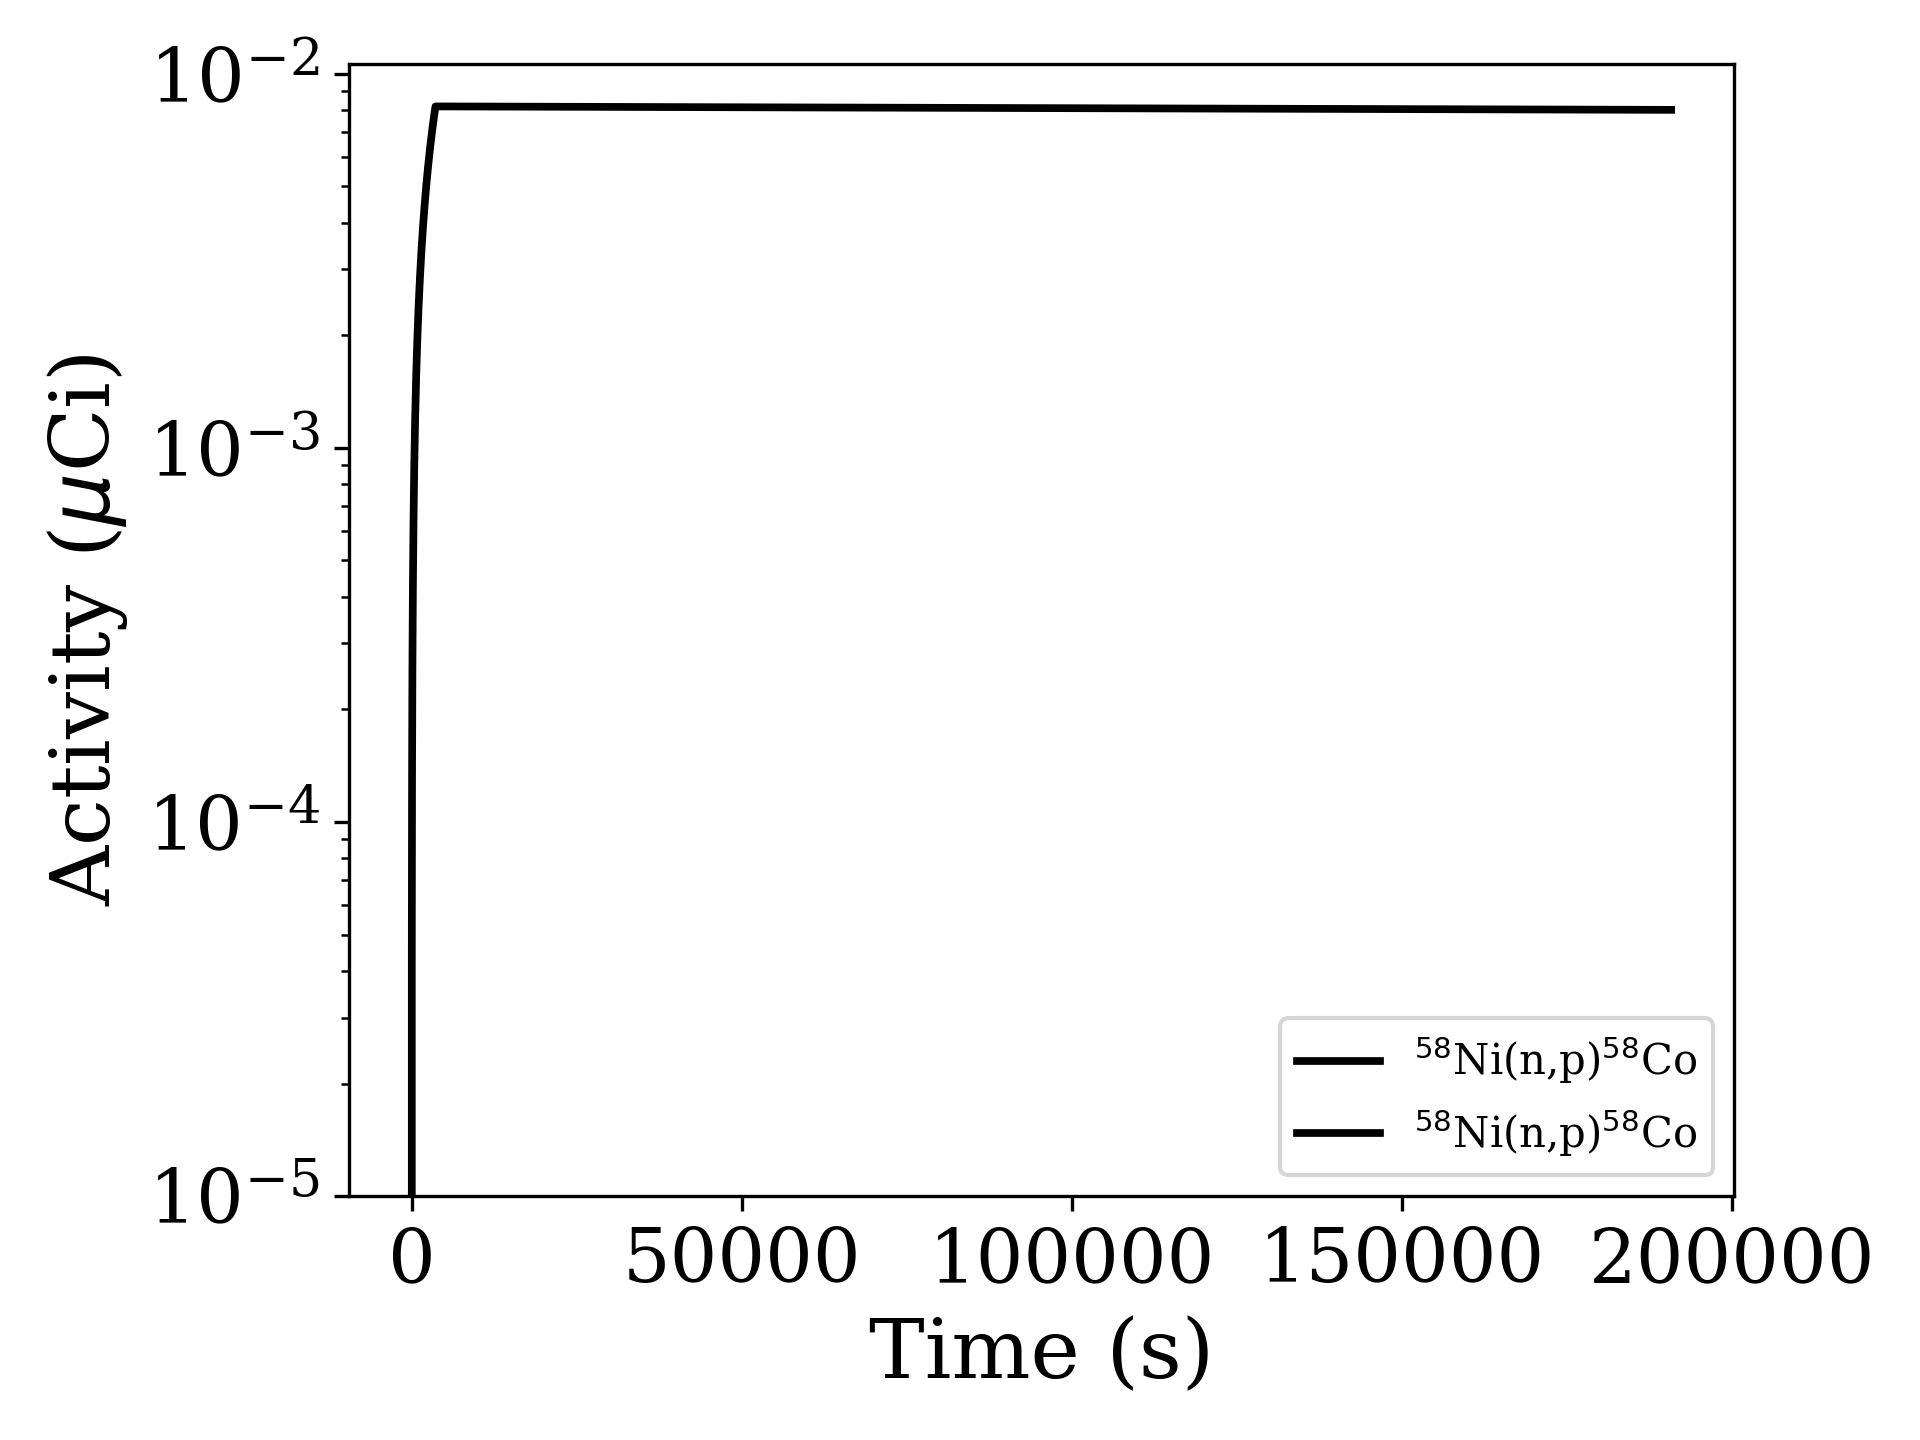
\includegraphics[width=.8\textwidth]{plot/Ni-58(n,p)Co-58_library1} 

  \caption{A subfigure}
  \label{fig:sub1}
\end{subfigure}%
\begin{subfigure}{.5\textwidth}
  \centering
     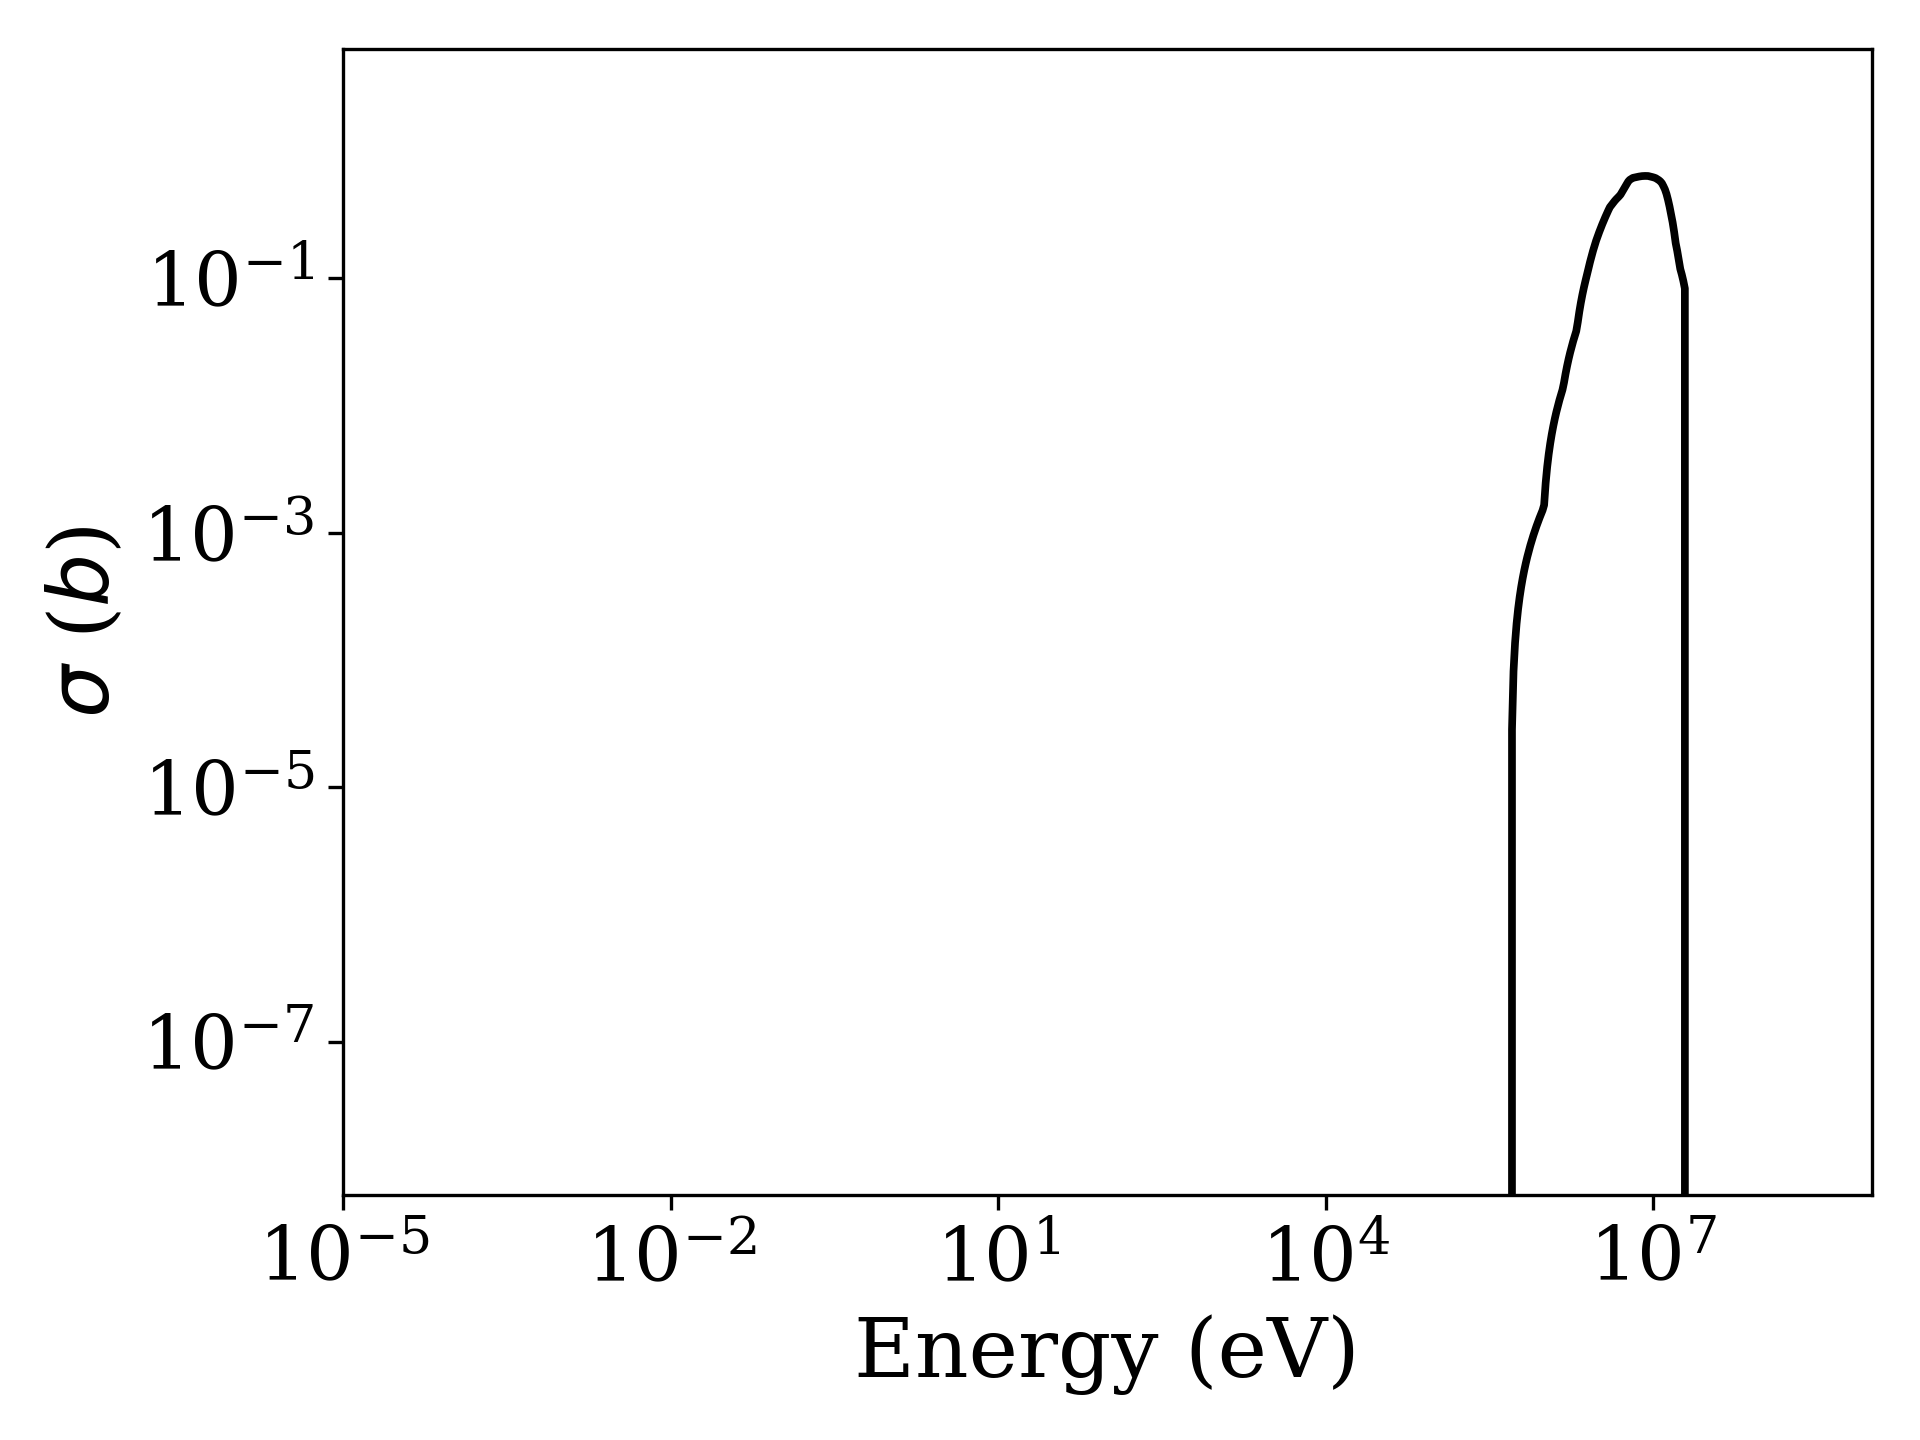
\includegraphics[width=.8\textwidth]{plot/Ni-58(n,p)Co-58} 

  \caption{A subfigure}
  \label{fig:sub2}
\end{subfigure}
\caption{A figure with two subfigures}
\label{fig:test}
\end{figure}

\begin{table*}[h]
\centering
\begin{tabular}{ |c|c|c|c|c|c|c| }
 \hline
 Reaction & T$_{1/2}$ & ROI (eV) & Important Gammas (keV) \\
 \hline 
 $^{58}$Ni(n,p)$^{58}$Co & 70.8 d & 1.94e+06, 7.88e+06 & 810.7593(0.9945) \\ 
\hline
\end{tabular}
\end{table*}
